\documentclass{article}

\usepackage{float}
\usepackage[pctex32]{graphics}
\usepackage{amssymb}
\usepackage{amsmath}
\usepackage{mathtools}
\usepackage{mathrsfs,relsize}
\usepackage[left=3cm,top=2cm,right=3cm,nohead,nofoot]{geometry}
\usepackage{latexsym}
\usepackage{pstricks}
\usepackage[nottoc]{tocbibind}
\usepackage{hyperref}
 

\parindent0pt
\parskip6pt
\pagestyle{empty}

\newcommand{\R}{{\mathbb R}}
\newcommand\Laplace{\mathlarger{\mathlarger{\mathscr{L}}}}
\title{Homework 4: Using Kaczmarz Iteration to Solve Inverse Laplace Transform as Linear Transformation}
\author{Duttaabhinivesh Devathi}
%content

\begin{document}
\maketitle
\tableofcontents
\section{Looking at the Problem}

Our goal is to solve the numerical inverse Laplace transform, where the Laplace transform is given by

\begin{equation}
\mbox{\Large\(
\mathscr{L} u(s) = \int_0^{\infty} e^{-st}u(t)dt,   s > 0.
\)}
\end{equation}

Recovering the function $u(t)$ is a challenge if we are given a noisy observation of the Laplace transformation, so we will test Kaczmarz Iteration.

\section{Setting Up The Problem}

\subsection{True Function}

The true function is a simple, piecewise linear function given by the following equation:

\begin{equation}
\mbox{\Large\(
  u(t) =
  \begin{cases}
  t & \text{if $ 0 <= t < 1$} \\
  \frac{3}{2} - \frac{t}{2} & \text{if $1 <= t < 3$} \\
  0 & \text{if $t >= 3$}
  \end{cases}
  \)}
\end{equation}

The function is plotted in Figure~\ref{fig:Piecewise}.

\begin{figure}[H]
    \centerline{
    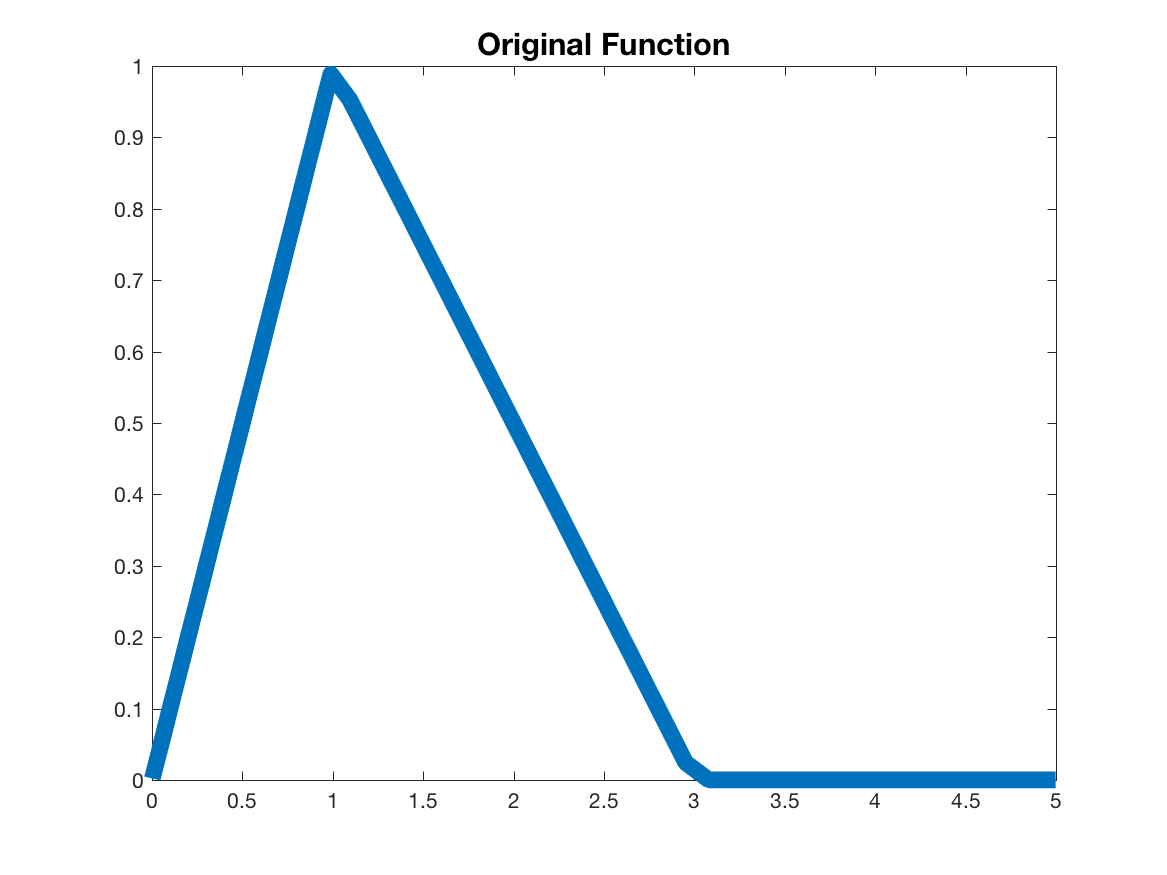
\includegraphics[height = 10 cm]{Piecewise.png}
    }
    \caption{\label{fig:Piecewise}The plot shows the piecewise function $u(t)$ from Equation (2).}
    
\end{figure}

\section{Laplace Transformation}

\subsection{Two Kinds}

The Laplace transform of $u(t)$, $\Laplace{u(s)}$ is computed twice. The first method of computing is analytic, using Equation (1). $\Laplace{u(s)}$ is given below

\begin{equation}
\mbox{\fontsize{17}{21.6}\(
\mathscr{L} u(s) = \frac{(2 - 3e^{-s} + e^{-3s})}{2s^{2}},   s > 0.
\)}
\end{equation}
 
 
The second version of the Laplace transform is given using a linear system using Gauss-Legendre quadrature rule of order n to approximate the integral associated with the Laplace transform. This is done so that we can apply Kaczmarz iteration to this inverse problem. To justify this approximation, we compute both the analytic and the approximated system to show that they are very close:

\begin{figure}[H]
    \centerline{
    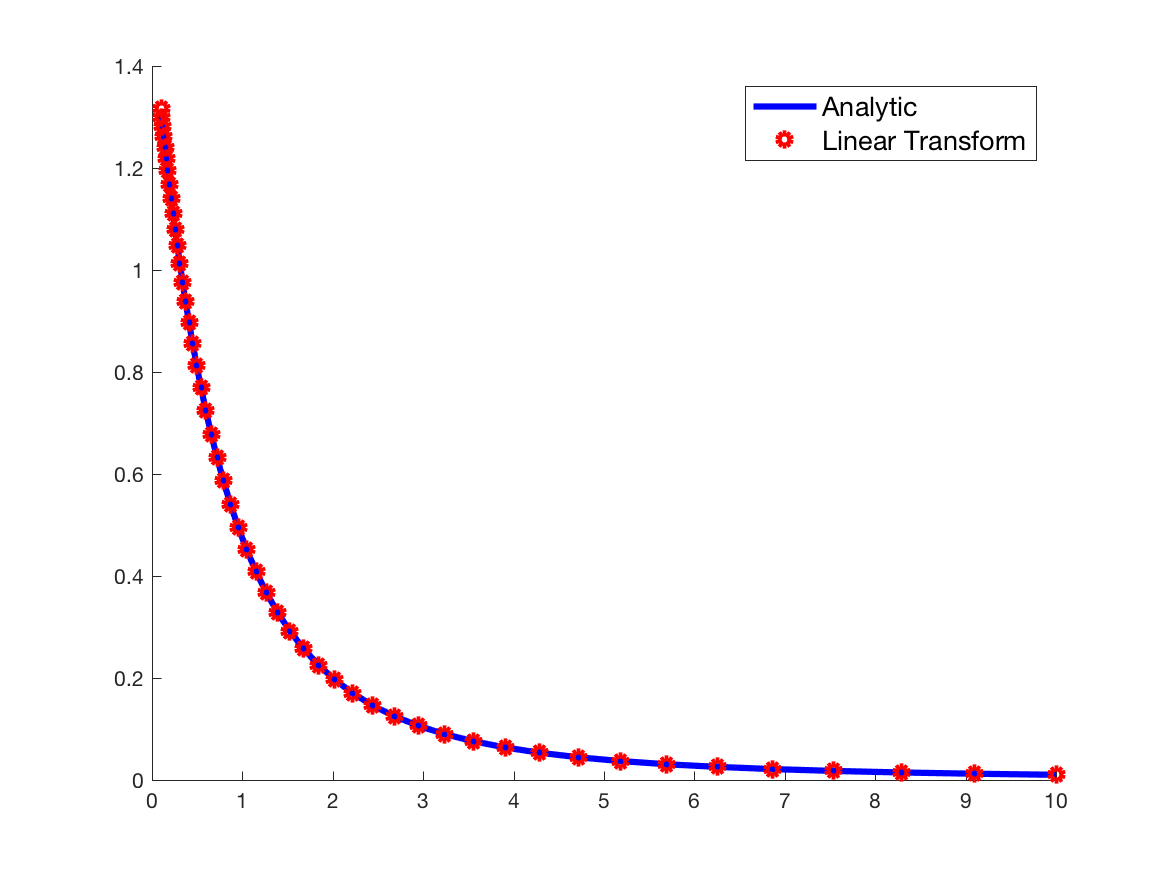
\includegraphics[height = 10 cm]{Comparison.png}
    }
    \caption{\label{fig:Comparison} This plot shows both the Analytic Laplace Transformation and the Gauss-Legendre Approximation plotted on top of one another. As you can see, they are very close.}
\end{figure}

\subsection{Discretization}

One point of information is the choice of the discretization. As seen in Figure~\ref{fig:Comparison} there is a denser discretization near 0 and sparser as you increase $s$. This is because as s gets smaller, there will be more information about the function $u(t)$ in $\Laplace{u(s)}$. So, we choose our discretization for s as follows:

\begin{equation}
\mbox{\fontsize{14}{24}
\(
    log_{10}s_j = -1 + \frac{2(j - 1)}{m - 1},   1 \leq j \leq m. 
\)
}
\end{equation}

\subsection{Matlab}

Here we will go over the code and parameters we use to set up the problem.

\subsubsection{Data Generation}

We want to compute the Laplace transform analytically as the \textit{noiseless exact data}. We choose our discretization size to be \texttt{$m = 50$} and use Equation (3). Here is the code:

\begin{verbatim}
%% Data Vector
m = 50;
ints = (1:m)';
s = 10.^(-1 + 2*(ints - 1)/(m - 1)); % discretization for s

% Laplace Transform, calculated analytically
Lu = @(s) (1./(2.*s.^2)).*(2 - 3.*exp(-s)+exp(-3*s));
b0 = Lu(s); % noiseless exact data
\end{verbatim}

\subsubsection{Discretization Points for t}

We compute this based on our bounds and our desired size of discretization for t from the piecewise function from Equation (1). We compute this using the Matlab function \texttt{GLquadrature.m} which is a Program to compute the abcissae and the weights of Gauss-Legendre's n-point quadrature.

We used $\mathsf{a = 0, T = 5, n = 60}$, for $\mathsf{1\leq k \leq n}$.

\begin{verbatim}
%% Discretization
a = 0; T = 5;%  bound on discretization
n = 60; % number of points
[t, w] = GLquadrature(a, T, n);
\end{verbatim}

\subsubsection{Computing Forward Matrix A}

As stated previously, we wish to approximate the Laplace Transformation by a Linear transformation. We compute that matrix here from the weights we got from \texttt{GLquadrature.m}.

\begin{verbatim}
A = repmat(w',m,1).*exp(-s*t'); % one-liner Hell yeah!
\end{verbatim}

The SVD's are plotted below in Figure~\ref{fig:Singular Values}.

\begin{figure}[H]
    \centerline{
    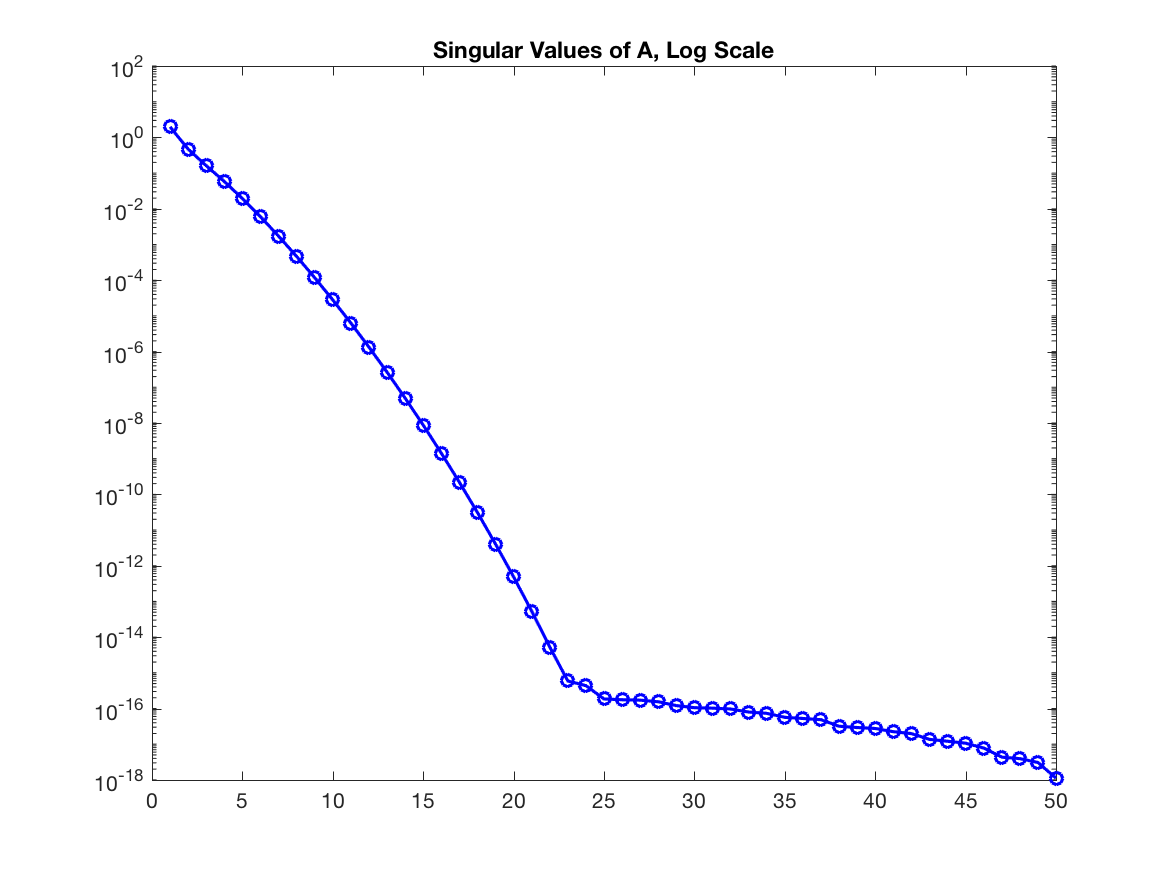
\includegraphics[height = 10 cm]{SingularValues.png}
    }
    \caption{\label{fig:Singular Values} The singular values of the forward matrix A, plotted on a log scale.}
\end{figure}

Upon inspection, we see that the relative error of the noiseless data and the transformed data is $5.237 \times 10^{-4}$, which is good enough. 

\subsection{Minimum Norm Solution}

To show the ill-posedness of the problem, here we show the Minimum Norm Solution using the back-slash command in Matlab.

\begin{figure}[H]
    \centerline{
    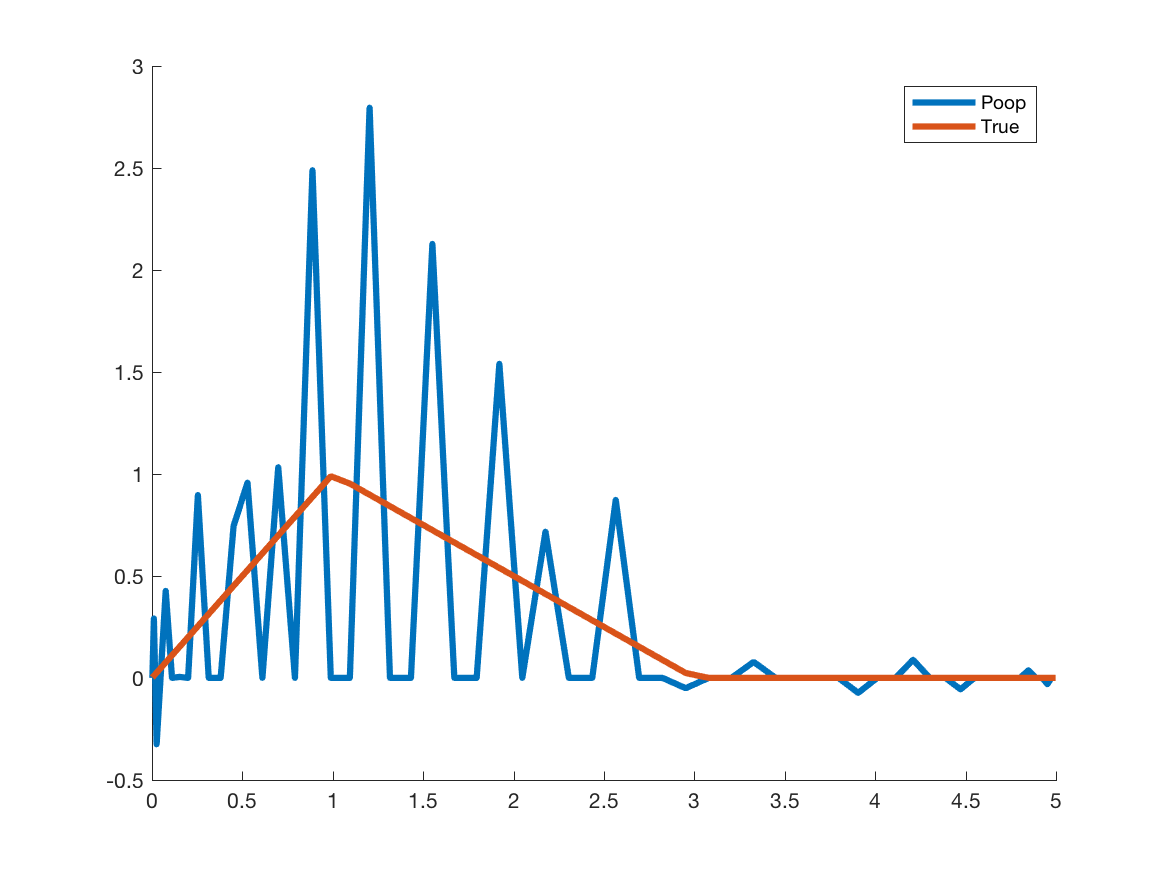
\includegraphics[height = 10 cm]{PoopSolution.png}
    }
    \caption{\label{fig:Poop Solution} The minimum norm solution plotted against the true solution.}
\end{figure}

\section{Kaczmarz Iteration}

\subsection{Noiseless Data}

We want to apply the Kaczmarz Iteration on the noiseless data to get a sense of how the iteration performs on this inverse problem. 

\begin{figure}[H]
    \centerline{
    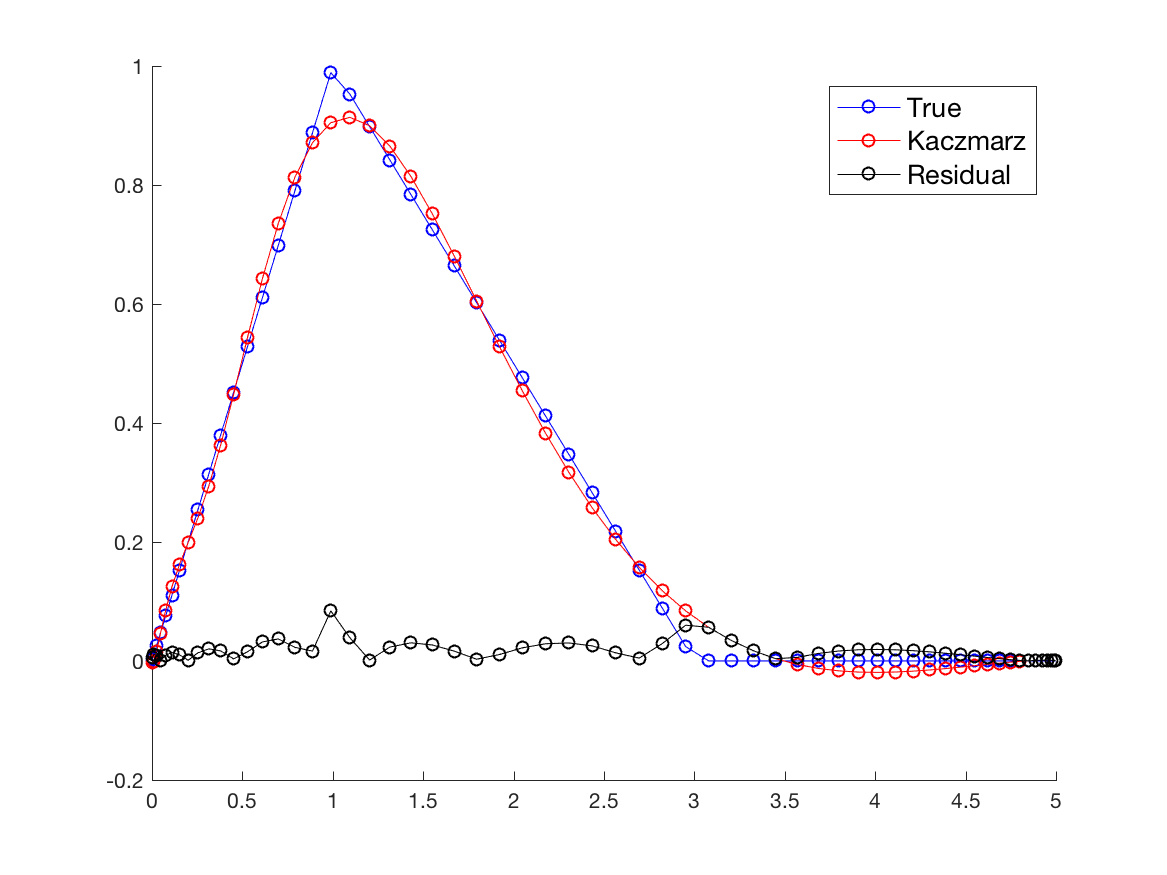
\includegraphics[height = 7 cm]{Noiseless.png}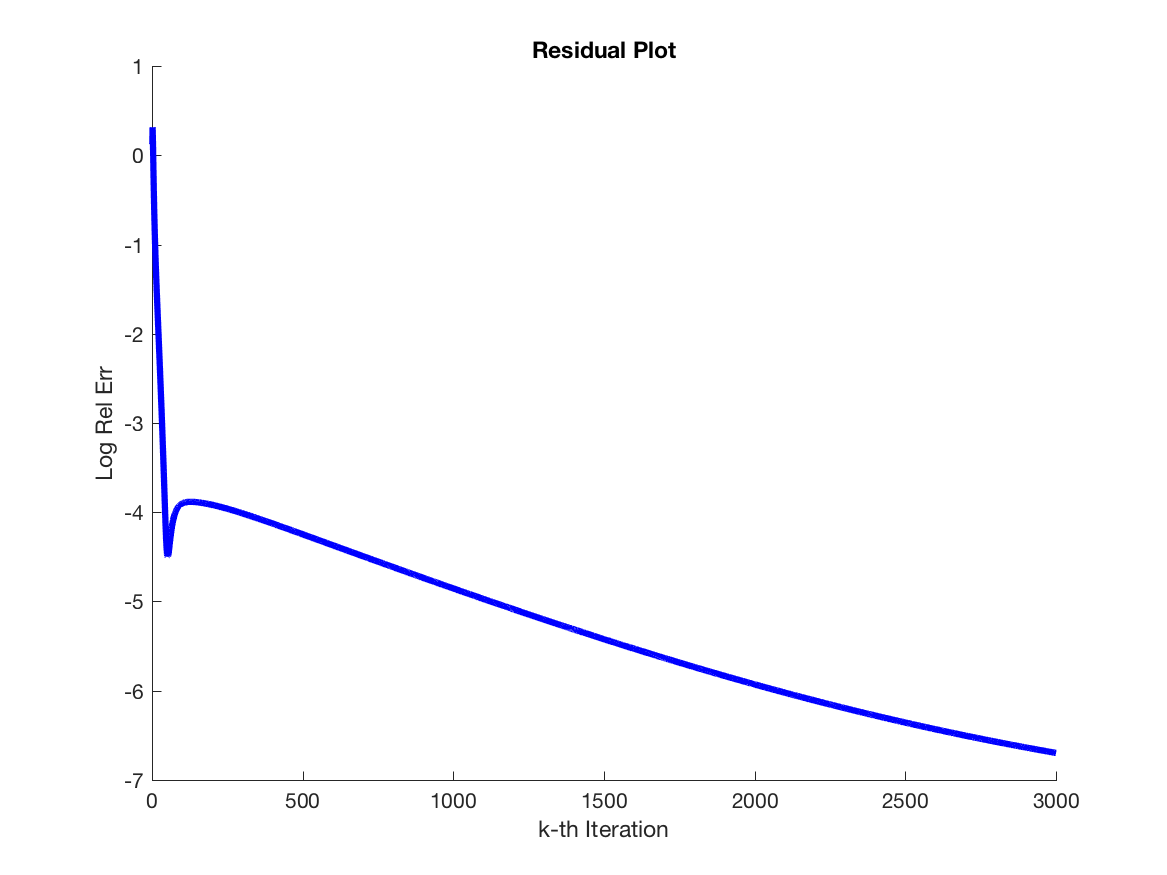
\includegraphics[height = 7cm]{Residuals-Noiseless.png}
    }
    \caption{\label{fig:Noiseless} The left panel shows the actual true solution in blue, given in Figure~\ref{fig:Piecewise} compared with the Kaczmarz solution in Red, while the black shows the norm of the residual at each $t_k$. The right panel shows the residual as the iteration increases.}
\end{figure}

As shown in Figure~\ref{fig:Noiseless}, the Kaczmarz Solution and the True solution are very close (a much better approximation than the minimum norm solution). It struggles at points where the function is not differentiable, such as $t_{k} = 1, 3$. This makes sense because these points are where the function $u(t)$ changes. 

Further, the residual curve has some interesting properties. After the first couple iterations, we see that there is a local minimum in the residual. Then there is a small uptick and gradually decreases as the iteration continues.

The Kaczmarz iteration algorithm is given in the Appendix under \texttt{Kaczmarz.m}, for reference.

\subsection{Adding Noise to Kaczmarz}

In the real world, we never see data that is noiseless. So, we wish to test Kaczmarz with noisy data. We vary the noise level $\sigma = 10^{-6},...,10^{-2}$ and look at the solutions.

\begin{figure}[H]
    \centerline{
    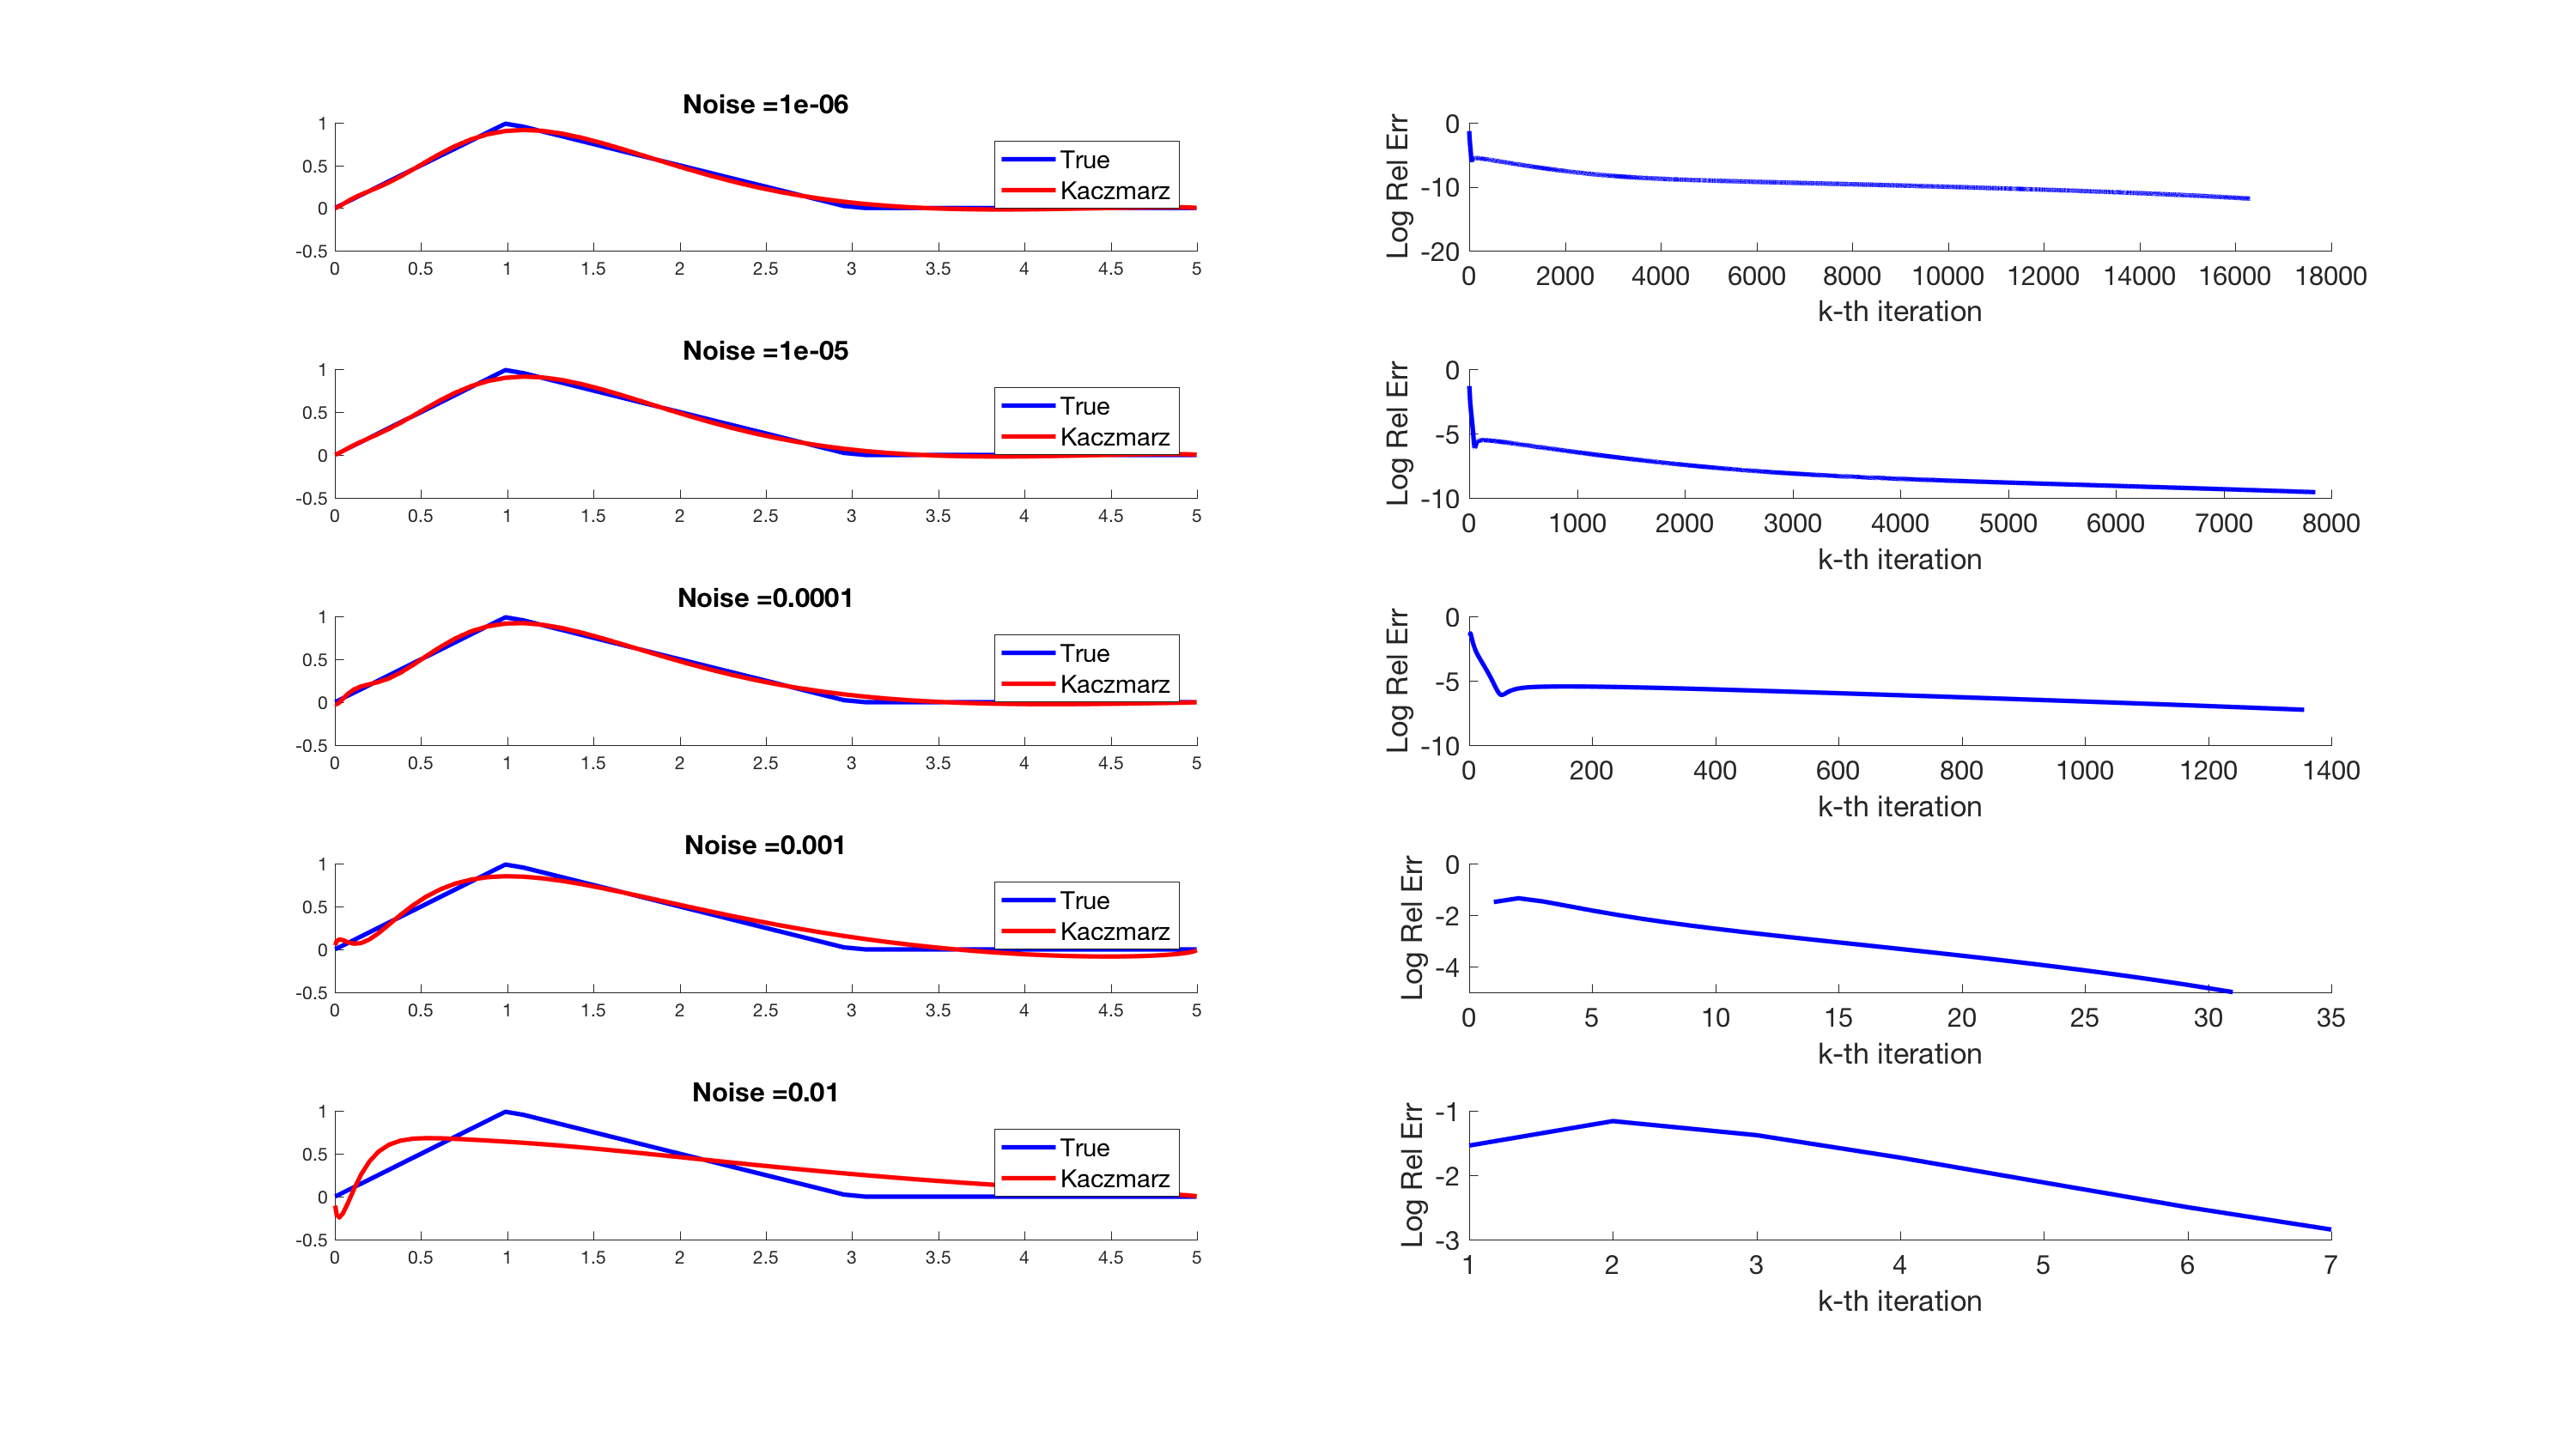
\includegraphics[height = 13 cm]{Iteration.png}
    }
    \caption{\label{fig:Iteration} The plots and the residual curves for varying the noise levels. The left panel shows the true solution plotted against the Kaczmarz iterative solution, for each given noise level.. The right panel shows the residual of the computed solution at each step.}
\end{figure}


Figure ~\ref{fig:Iteration} shows the solutions and residual plots. As you can see, for small noise levels $\sigma = 10^{-6},...,10^{-3}$, the solution is not that far off from the actual true solution. However, once the noise level hits $10^{-2}$, there is too much noise for the data to be interpreted properly. 

Further, the point at which each curve stops in the residual curve is where the curve reaches its discrepancy based on the Morozov Discrepancy Principle. As you can see, if you increase the noise level by 10, then the solution converges at an order of magnitude smaller number of iterations. Further, you you see that the same structure of the residual curve (having a local min quickly, and a small uptick followed by a gradual decrease) is apparent in the smaller values of noise. As you increase noise however, this becomes less true because it's harder to fit the data.

\section{Conclusion}

Overall, the Kaczmarz Iterative method to solve Inverse Problems proved to be effective on the notoriously ill-posed inverse Laplace Transform. While the iteration performed well to provide a general outline of the true solution, more work needs to be done to do analysis of this method on other Laplace transforms. Further, it seems that there needs to be correcting measures taken for points that are non-differentiable or where a curve has a high curvature, as these are the points where the Kaczmarz solution has the highest error margin. Perhaps this is because Kaczmarz Iteration prefers the data to be continuous, after all who doesn't. 

\section{Appendix}

\subsection{\texttt{GLquadrature.m}}
\begin{verbatim}
% FUNCTION program [x,w] = GLquadrature(a,b,n)
% ----------------------------------------------------------------------------
% Program to compute the abcissae and the weights of Gauss-Legendre's n-point
% quadrature, when the lower and upper limits of the integration are given.
% This algorithm is from Numerical Recipes page 125.
% INPUT  a,b : lower and upper limits of the integration
%         n  : number of division points in the integration
% OUTPUT  x  : (n,1)-vector listing the integration points (abscissae)
%         w  : (n,1)-vector listing the quadrature weights
% ----------------------------------------------------------------------------
function [x,w] = GLquadrature(a,b,n)

tol = 1e-15 ;                            % tolerance for Newton's method
m = (n+1) / 2 ;
xm = 0.5*(b+a) ;
xl = 0.5*(b-a) ;
for i=1:m
   % approximations of the roots
   if i == m
      z = 2*tol ;                        % right value of z is zero
   else
      z = cos(pi*(i-0.25)/(n+0.5)) ;
   end
   z1 = 0 ;
   while ( abs(z-z1) >= tol )
   % Newton's method for roots of Legendre's polynomials
      p1 = 1 ; p2 = 0 ;
      for j = 1:n
         p3 = p2 ;
         p2 = p1 ;
         p1 = ((2*j-1)*z*p2-(j-1)*p3)/j ; % Legendre's polynomial at point z
      end
      pp = n*(z*p1-p2)/(z^2-1) ;   % derivative of Legendre's polynomial at z
      z1 = z ;
      z = z1-p1/pp ;                   % Newton's method
   end
   x(i) = xm-xl*z ;                    % abscissae
   x(n+1-i) = xm+xl*z ;
   w(i) = 2*xl/((1-(z^2))*(pp^2)) ;    % and weights
   w(n+1-i) = w(i) ;
end
x = x'; w = w';
\end{verbatim}

\subsection{\texttt{Kaczmarz.m}}
\begin{verbatim}
function [discrs,u] = Kaczmarz(A,b,noiselev)
[m,n] = size(A);
u = zeros(n,1);
k = 0; % Iteration Counter
discr = Inf; % residual
MAX_ITER = 3000; % So we don't kill our CPU
discrs = zeros(MAX_ITER,1); % store residual at each iteration 
while(k < MAX_ITER && discr > noiselev)
    for j = 1:m
        aj = A(j,:)';
        % Using the Kaczmarz Projection to compute the next solution
        u = u + (1/norm(aj))^2*(b(j) - aj'*u)*aj;
    end
    k = k+1;
    
    % Compute Relative Error of Residual
    discr = norm(b - A*u)/norm(b);
    discrs(k) = discr;
end

% Truncate so we don't get values after iteration stops
discrs = discrs(1:k); 
end
\end{verbatim}

\end{document}